\documentclass[oneside]{book}
\usepackage{url,verbatim,fancyvrb}
\usepackage{pifont}
\usepackage[latin1]{inputenc}
\usepackage[pdftex]{graphicx}
\usepackage[authoryear]{natbib}
\usepackage{color,gretl}
\usepackage[letterpaper,body={6.3in,9.15in},top=.8in,left=1.1in]{geometry}
\usepackage[pdftex,hyperfootnotes=false]{hyperref}
\usepackage{dcolumn,amsmath,bm}

\newcommand{\ttusage}[1]{\textit{example}: \quad \texttt{#1}}
\newcommand{\vbusage}[0]{\textit{example}: \quad}

\setcounter{secnumdepth}{2}

\bibliographystyle{gretl}

%% \pdfimageresolution=120
\hypersetup{pdftitle={Gretl Function Package Guide},
            pdfsubject={Using and writing gretl function packages},
            pdfauthor={Allin Cottrell and Riccardo (Jack) Lucchetti},
            colorlinks=true,
            linkcolor=blue,
            urlcolor=red,
            citecolor=steel,
            bookmarks=true,
            bookmarksnumbered=true,
            plainpages=false
}

\begin{document}

\VerbatimFootnotes

\setlength{\parindent}{0pt}
\setlength{\parskip}{1ex}
\setcounter{tocdepth}{1}

%% titlepage

\thispagestyle{empty}

\begin{center}
\pdfbookmark[1]{Gretl Function Package Guide}{titlepage}

\gtitle{Gretl Function Package Guide}

{\large \sffamily
Allin Cottrell\\
Department of Economics\\
Wake Forest University\\

\vspace{20pt}
Riccardo (Jack) Lucchetti\\
Dipartimento di Scienze Economiche e Sociali\\
Universit� Politecnica delle Marche\\

\vspace{20pt}
\input date
}

\end{center}
\clearpage

%% end titlepage, start license page

\thispagestyle{empty}

\pdfbookmark[1]{License}{license}

\vspace*{2in}

Permission is granted to copy, distribute and/or modify this document
under the terms of the \emph{GNU Free Documentation License}, Version
1.1 or any later version published by the Free Software Foundation
(see \url{http://www.gnu.org/licenses/fdl.html}).

\cleardoublepage

%% end license page, start table of contents
\pdfbookmark[1]{Table of contents}{contents}

\pagenumbering{roman}
\pagestyle{headings}

\tableofcontents

\clearpage
\pagenumbering{arabic}
%\setcounter{chapter}{-1}

\chapter{Introduction}
\label{chap:intro}

\section{The purpose of function packages}
\label{sec:purpose}

The primary purpose of gretl function packages is to add estimators,
hypothesis tests or other analytical procedures to gretl's repertoire
of built-in procedures. While function packages may also be used for
other purposes (e.g.\ pedagogy, replication exercises), those made
available via the gretl server are expected to extend gretl's
functionality in non-trivial ways.

For an extended discussion of the rationale for such packages see
``Extending gretl: addons and bundles'' \citep{addons-bundles}. Note,
however, that the distinction between regular packages and ``addons''
in that document has become somewhat blurred, as regular packages have
gradually acquired many of the rights and responsibilities previously
confined to official gretl ``addons''. On the rights side, regular
packages are now able to hook into the gretl GUI; on the
responsibilities side, contributed packages are now subject to
(minimal) vetting before they can appear in the public download area
on the gretl server.
  
\section{The form of function packages}
\label{sec:pkgform}

The core component of a gretl function package---in simpler cases,
the sole component---is a \textsf{gfn} file. This is an XML file
conforming to the Document Type Definition \texttt{gretlfunc.dtd},
which is supplied in the gretl distribution and can also be found in
gretl CVS.\footnote{See
  \url{http://gretl.cvs.sourceforge.net/viewvc/gretl/gretl/share/functions/gretlfunc.dtd?view=log}.}
Such files contain
\begin{itemize}
\item the hansl code for at least one function;
\item various items of metadata (author, version, date, etc.);
\item help text for the function(s), or a pointer to help in
  PDF format; and
\item a sample script that illustrates a call to the packaged
  function(s). 
\end{itemize}

While it is possible in principle to create and edit a \textsf{gfn}
file ``manually'', using a suitable text editor, this is not
recommended. Gretl provides tools (both command-line and GUI) to create
and maintain package files, such that authors are not required to
mess with raw XML.

We will refer to packages that consist of a gfn file alone as ``simple
packages'' (the included hansl code may not be simple, but the
structure is). 

The alternative to a simple package we will call a ``zip package''.
Such packages take the form of a \textsf{PKZIP} archive containing a
\texttt{gfn} file along with other materials, which may include PDF
documentation (in place of plain text help), data needed by the
package for internal use (for example, tables of critical values for
some test statistic), and/or extra data files or scripts intended to
supplement the required sample script. Zip packages can be built using
command-line tools or with the help of the gretl GUI.

One point to note about zip packages is that the \textsf{PKZIP}
wrapper is actually just a storage and transport format. When such a
package is installed, it is unpacked in a suitable location. Further
details on this package format can be found in
chapter~\ref{chap:zipfile}.

\section{Using this document}

Chapter~\ref{chap:users} gives an account of function packages from
the user's point of view. Even those who are familiar with packages
might want to take a look, since there are some finer points that
might not be totally evident. Moreover, there are several changes
and enhancements in recent gretl.

Chapter~\ref{chap:authors} gives a walk-through of the means of
creating, refining and publishing function packages, both via
the command-line and via the GUI.

Chapters~\ref{chap:specfile} and \ref{chap:zipfile} provide reference
material on the details of package specification and structure, along
with some tips on usage.

%%%%%%%%%%%%%%%% chapter break %%%%%%%%%%%%%%%%%

\chapter{For package users}
\label{chap:users}

\section{Acquiring a package}
\label{sec:acquire}

The first thing is finding out what packages are available. At
present, most packages that are likely to be of interest are contained
in gretl's official repository. These have passed a minimal checking
procedure on the part of the gretl development team, designed to
ensure that they are usable with the current version of gretl. This
does not mean, however, that they are guaranteed to be bug-free, or to
deliver accurate results; those responsibilities rest on the shoulders
of the package authors.

Some authors may choose to make their packages available via other
means. In that case, once the user has the package file available,
either as a \textsf{gfn} file or a \textsf{zip} file (see
section~\ref{sec:pkgform}), the package can be installed using
the instructions below (section \ref{sec:cli-install}).

\subsection{Searching the package repository}
\label{sec:repo}

The list of available function packages can be browsed from within
gretl itself or via the web.

From within gretl, you can call up a list of packages on the gretl
server by selecting the menu item ``Tools, Function packages, On
server''. This provides a convenient interface for upgrading your
packages, adding new ones, and deleting any that you don't
need. Alternatively, if you're only interested in browsing the
repository, you can visit the web interface at Wake Forest
University.\footnote{See
  \url{http://ricardo.ecn.wfu.edu/gretl/cgi-bin/gretldata.cgi?opt=SHOW_FUNCS}.}

If you're looking for some specific functionality (``I was told that
gretl can do such-and-such, but you need to install an additional
package''), a short ``description'' field is provided. \textbf{JEL
  codes should be on their way}


\subsection{Installing a package via the GUI}

We'll use as an example Ignacio D\'iaz-Emparanza's \textsf{GHegy}
package.  Suppose you've read Ignacio's excellent paper
\citep{Ignacio-HEGY} and you'd like to use his results. You were
told a gretl package is available. Here's what you do.

Open gretl, and select ``Tools, Function packages, On server''. Since
the package deals with seasonal unit roots, you'll probably want to
look for the word ``seasonal''. After typing \texttt{seasonal} in the
top-right search box and hitting the \textsf{Enter} key a few times,
you find what looks like it (Figure~\ref{fig:ghegy-lst}).

\begin{figure}[htbp]
\begin{center}
  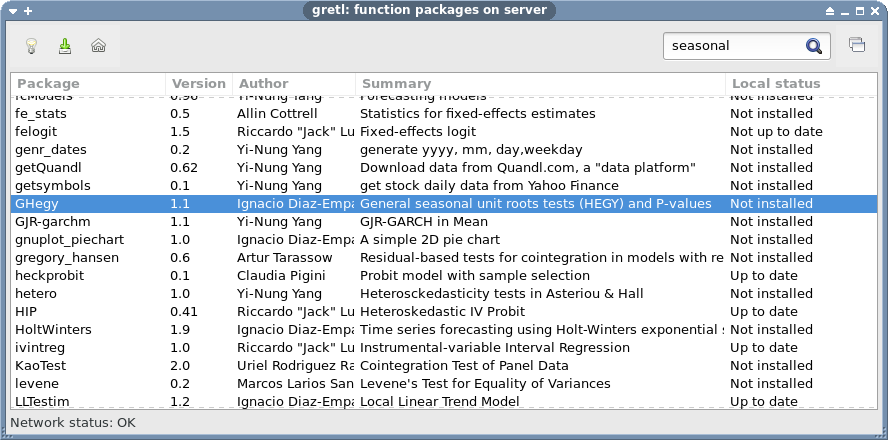
\includegraphics[width=0.8\textwidth]{figures/ghegy-lst.png}
\end{center}
\caption{Find GHegy in the package browser}
\label{fig:ghegy-lst}
\end{figure}

To make sure this is really what you want, you can get more
information on the package, either by clicking on the ``Info'' icon
(top-left), or by right-clicking on the package entry and selecting
\textsf{Info} from the context menu. You'll be presented with a window
like Figure~\ref{fig:ghegy-info}.

\begin{figure}[htbp]
\begin{center}
  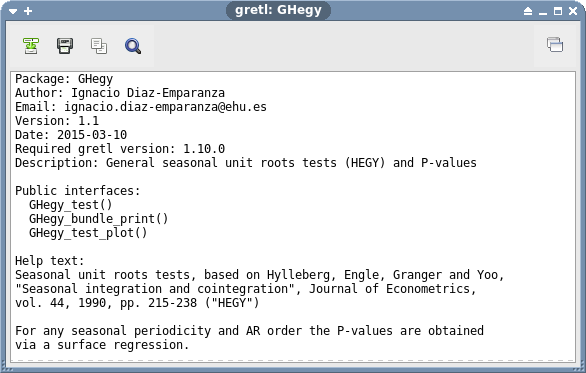
\includegraphics[width=0.6\textwidth]{figures/ghegy-info.png}
\end{center}
\caption{Get more info on GHegy}
\label{fig:ghegy-info}
\end{figure}

Yes, this definitely looks like it. At this point, all you have to do
is install the package: click on the ``Install'' icon in the browser
window, or, again, right-click on the package entry. Gretl will now
download the package from the server at Wake Forest University (we
assume you have an Internet connection) and install it.

\begin{figure}[htbp]
\begin{center}
  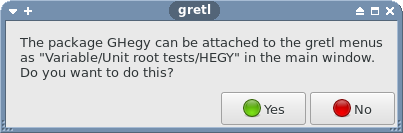
\includegraphics[width=0.4\textwidth]{figures/ghegy-menu.png}
\end{center}
\caption{Let GHegy attach to a menu?}
\label{fig:ghegy-menu}
\end{figure}

The final step of your installation is shown in
Figure~\ref{fig:ghegy-menu}.  Function packages may offer the option
of integrating into gretl's GUI menus: in this case, the author chose
to make it available among the other unit-root tests that gretl
provides natively. You may choose to accept this option (which makes
it handy to use the package from gretl's graphical interface) or not,
if you don't want to clutter up your menus with anything more than the
essential entries. Even if you say ``No'' here, however, the package
will still be available to you from the GUI interface---it just won't
have a dedicated menu entry. But note, this is not just a one-time
option; see section~\ref{manage-menus} for an account of how to
add or remove installed packages from gretl's menus.\label{pg:menu-hook}

Suppose, for now, you say ``Yes'' to \textsf{GHegy}'s offer of a menu
attachment. Then the HEGY unit-root test should be available where
you'd expect to find it (Figure~\ref{fig:ghegy-hook}).\footnote{You
  used to have to restart the program to get such dynamic menu items
  to appear, but from gretl 1.10.2 that's no longer necessary.}

\begin{figure}[htbp]
\begin{center}
  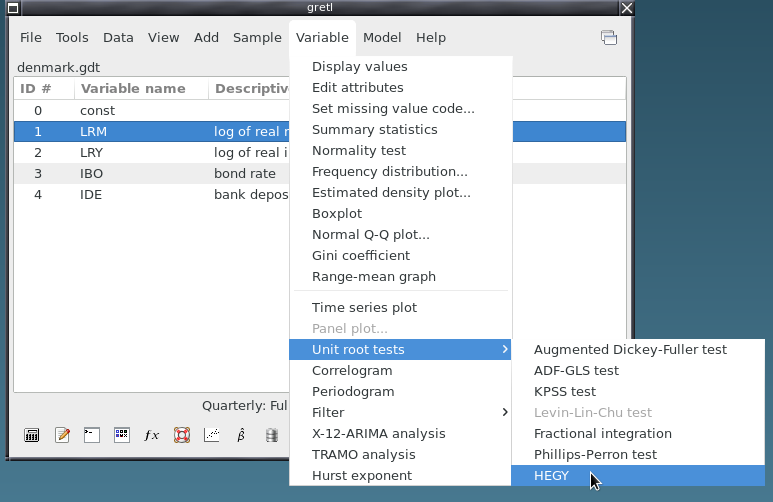
\includegraphics[width=0.8\textwidth]{figures/ghegy-hook.png}
\end{center}
\caption{The added menu item}
\label{fig:ghegy-hook}
\end{figure}

\subsection{Installing a package via the command line}
\label{sec:cli-install}

An alternative mechanism is provided by gretl's \cmd{install} command,
which can be invoked in the gretl console or in the command-line
program \app{gretlcli}. This command has three modes:

\begin{itemize}
\item If you just type, for example,
%
\begin{code}
install GHegy
\end{code}
%
the presumption is that you mean to install a package named
\textsf{GHegy} (either \texttt{.gfn} or \texttt{.zip}, that will be
determined automatically) from the gretl server. So, another way
of doing what we just walked through, if you know in advance exactly
what you want.
\item Suppose a colleague has given you a link to a function package
  that's not on the gretl server. Then you can download and install it
  on your own machine using the full URL, as in
%
\begin{code}
install http://somewhere.net/gretl/splendid.gfn
\end{code}
%
\item Finally, suppose you have somehow got a copy of a function
  package independently of gretl: it's on your computer but not
  installed.  Then, to install it you want the \option{local} option
  (and you need to know the path to the file). So you might type
%
\begin{code}
install /Users/Me/Downloads/splendid.gfn --local
\end{code}
%
\end{itemize}

\subsection{Updating a package}

Updating packages is easily done via the GUI. Look back at
Figure~\ref{fig:ghegy-lst}: in the right-most column of the browser
for ``packages on server'' you'll see a note of the local status of
each available package, either ``Up to date,'' ``Not installed'' or
``Not up to date.'' (It may be necessary to expand the browser window
or scroll to the right in order to see this column.) It's a good idea
to visit this listing from time to time; if an installed package is
marked as not up to date, just click the Install button to update it.

\section{Using function packages: the basics}

You can call up a browser window for your installed functions via the
main-window menu item ``Tools, Function packages, On local machine,''
or by clicking the ``\textit{fx}'' button on the toolbar at the foot
of the main window. The function-browser window has quite a rich set
of toolbar buttons and right-click context menu choices. If you're not
sure what a button might do, try mousing over it to get a ``tooltip.''
If you're still not sure, you might just try clicking it---gretl won't
do anything destructive without asking for confirmation first!

We'll discuss some of the less obvious choices in the window later,
but we would encourage you to explore.

\subsection{Using packages via scripting}

If you're interested in calling a function package via script you'll
probably want to examine its ``sample script.'' Hopefully this should
provide a useful template. Opening the sample script is one of the
options on right-clicking an installed package in the browser for
functions ``on local machine'' (see above).  Of course you should also
read the help text for the function you want to call.

You'll want to start your script by using the \cmd{include} command
to load the package in question, as in
%
\begin{code}
include GHegy.gfn
\end{code}

Note that even if a package comes in zip format, it's the \texttt{gfn}
file (which will be unpacked on installation) that you need to
include. It will always have the same basename as the zip package that
contained it.

The only effect of the \cmd{include} command above is to make the
functions contained in the package available to you. To use them, you
call them as if they were native gretl functions. So, for example, the
sample script for \textsf{GHegy} contains the following commands:

\begin{code}
include GHegy.gfn
open data9-3.gdt

# Tests with constant + dums + trend and fixed AR order 4, 
# without printing the regression
bundle H1 = GHegy_test(reskwh, 0, 4, 3, 0)

# Tests with constant + dums, AR order determined by BIC with 
# a maximum of 10, printing the regression
bundle H2 = GHegy_test(reskwh, 2, 10, 2, 1)
\end{code}

The purpose of the first two commands is obvious and needs no
comment. However, the two invocations of the \cmd{GHegy\_test}
function may not be totally transparent. In general you should expect
some documentation on (a) which functions are contained in the package
and (b) their syntax: the parameters they accept, what they do, what
they return.\footnote{This is something that the package authors are
  completely in charge of: we, as the gretl development team, try to
  ensure that packages obtained via the gretl server contain at least
  minimal documentation, but we cannot guarantee anything more.}  To
find this, go to the list of locally-installed packages and click on
the ``Info'' icon. A text box will appear showing the documentation
provided by the package author. in the \textsf{GHegy} case, for
example, not only are we told all we need to know about the
\cmd{GHegy\_test} function, but we also discover that the package
contains two additional functions we can use, namely
\cmd{GHegy\_bundle\_print} and \cmd{GHegy\_test\_plot}.  So, for
example, we could use the latter to enhance Ignacio's sample script,
appending the line
%
\begin{code}
GHegy_test_plot(&H2)  
\end{code}
%
Running it will then produce a graphic similar to the one displayed in
Figure~\ref{fig:ghegy-plot}.

\begin{figure}[htbp]
  \centering
  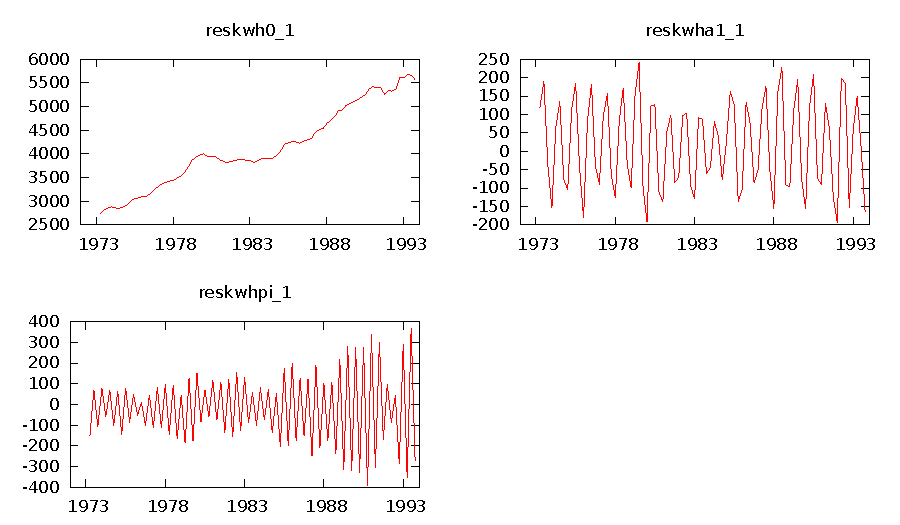
\includegraphics{figures/ghegy-plot}
  \caption{Output of the \cmd{GHegy\_test\_plot} function}
  \label{fig:ghegy-plot}
\end{figure}

Some packages may contain a substantial number of function or have
other characteristics such that the package authors may prefer
supplementing the help text with documentation in PDF format. This is
the case, for example, of the \textsf{DPB} package
\citep[see][]{DPBwp}. If a pdf file is available, you will have a
``Help'' icon available among those of the list of locally-installed
packages, and clicking on it should load it in your default pdf
reader.

Other than that, there's not much to say here. For help on scripting
in general, see the \textit{Hansl Primer} \citep{hansl-primer}.

\subsection{Using packages via the GUI}
\label{sec:gui-using}

Of course, if a package offers to attach to a gretl menu, and you
accepted that offer when you installed the package (see
p.~\pageref{pg:menu-hook}) then you should know where to find it.
But if a package doesn't have its own place in the menus, the
package browser is the place to go to invoke it by GUI means.

You can launch a package by double-clicking on it. What exactly
happens here depends on whether the package's data requirement is
met. Most packages require that a dataset is open, and some have more
specific requirements (time series data, or panel data). 

If you have a suitable dataset in place you will get a dialog box to
specify arguments to the function, much as you would with a built-in
gretl procedure. (However, if the package offers more than one public
interface you may get an initial dialog asking you to choose a
particular function to call.) If the package's data requirement is not
met, you'll be told what's wrong and asked if you'd like to run the
sample script. This should load suitable data and ``demo'' the
package.\footnote{By the way, if a package's sample script does not
  run correctly you are encouraged to report that to the author of the
  package or the \texttt{gretl-users} mailing list. Although gretl
  function packages carry no warranty it is supposed to be an absolute
  requirement that the sample script runs OK.}

\begin{figure}[htbp]
  \centering
  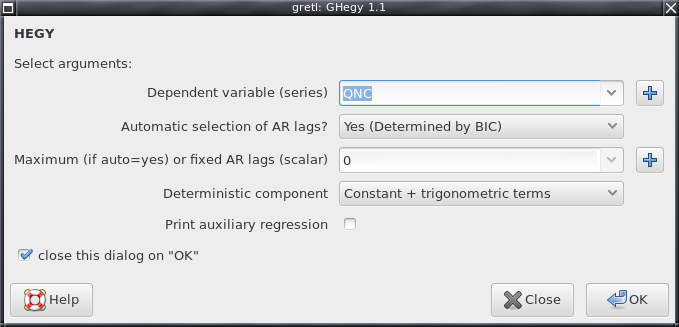
\includegraphics[width=0.7\textwidth]{figures/ghegy-call}
  \caption{GUI call to the \textsf{GHegy} packge}
  \label{fig:ghegy-call}
\end{figure}

Figure~\ref{fig:ghegy-call} illustrates a function-call dialog, this
one put up by the \textsf{GHegy} package. Each argument to the
function is represented by either a drop-down selector or a check
box. Note that the ``\textsf{+}'' button next to a selector allows you
to define a new variable as an argument if you
wish. Figure~\ref{fig:ghegy-output} then shows part of the output from
this call.

\begin{figure}[htbp]
  \centering
  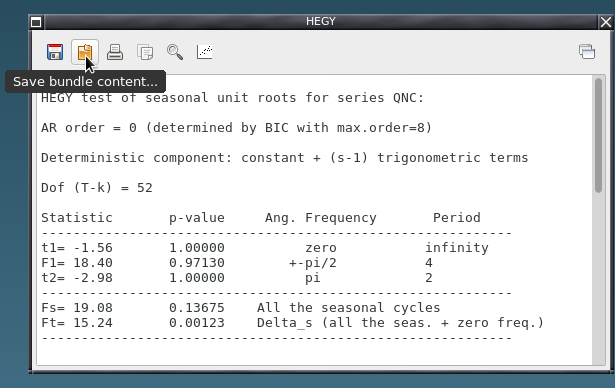
\includegraphics[width=0.7\textwidth]{figures/ghegy-output}
  \caption{Output window from call to \textsf{GHegy}}
  \label{fig:ghegy-output}
\end{figure}

We have moved the mouse pointer over the ``bundle'' icon in the
toolbar of this window ro reveal the tooltip, ``Save bundle content.''
What's going on here is that \textsf{GHegy} has constructed a gretl
bundle containing various details of the unit root test, and we can
extract these details if we wish. Package authors: for an account of
how to do this sort of thing see section~\ref{sec:idioms}.


\section{Some finer points}
\label{sec:finer}

\subsection{Managing menu attachments}
\label{manage-menus}

We mentioned above that you can revise your initial choice of whether
or not to have a function package insert itself into the gretl
menus. We'll now explain how.

Again, start from the browser for packages ``on local machine''. One
of the buttons on the toolbar is a ``\textsf{+}'' icon (with tooltip
``Add to menu''). This button should be active when you select a
package which (a) offers a menu attachment but (b) is not currently
attached. Click it and you'll get the sort of dialog shown in
Figure~\ref{fig:ghegy-menu}; say ``Yes'' to attach the package to the
specified menu.

To go the other way---that is, remove a package from a menu---use the
button with the ``Preferences'' icon (tooltip ``Package
registry''). This brings up a window showing the packages that are
currently attached to menus (Figure~\ref{fig:pkg-registry}). For each
package you can see whether its attachment is in the main gretl window
or in model windows (at present these are the only two possibilities),
as well as the specific ``path'' to the menu item. To remove a package
from the menus, use the delete button or the right-click
menu. Removing a package from the menu system does not delete or
disable the package, it just means it won't have its own menu
item---which is easily reversed, as we have just seen.

\begin{figure}[htbp]
  \centering
  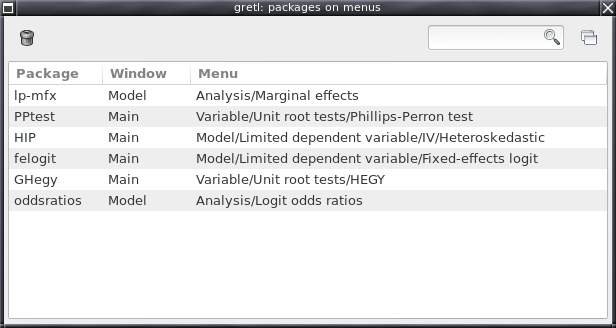
\includegraphics[width=0.8\textwidth]{figures/pkg-registry}
  \caption{The GUI package ``registry'': from here you can remove
    dynamic menu items}
  \label{fig:pkg-registry}
\end{figure}

Changes made in this way will have immediate effect on main-window
menus; the effect on model-window menus will be apparent only for
newly opened windows.

\subsection{What does ``installed'' mean?}
\label{sec:installed}

We've talked about installing packages, but what exactly does it mean
for a package to be installed? Basically, it means that the package
file(s) are placed in one or other of two standard locations where
gretl should always be able to find them automatically---for example,
in response to the command ``\texttt{include mypkg.gfn}'' without any
path specification.

These two standard locations are the ``system'' and ``per-user'' gretl
function directories. In each case we're talking about a subdirectory
named \texttt{functions}, the actual path to which differs by platform
(and on MS Windows, by national language).

On an English-language Windows installation typical values are, for
the system and per-user paths respectively,
%
\begin{code}
C:\Program Files\gretl\functions
C:\Users\login\AppData\Roaming\gretl\functions
\end{code}
%
where ``login'' is a placeholder for your username. On Linux they are
likely to be
%
\begin{code}
/usr/share/gretl/functions
$HOME/.gretl/functions
\end{code}
%
and on Mac OS X
\begin{code}
/Applications/Gretl.app/Contents/Resources/share/gretl/functions
$HOME/Library/Application Support/gretl/functions
\end{code}
%
where
\verb|$HOME| is your ``home'' directory, which is always defined on
Linux and OS X.

However, you don't need to guess at these locations: in the gretl
console you can do
%
\begin{code}
eval $gretldir
eval $dotdir
\end{code}
%
to get the respective base directories on your system: append
\texttt{functions} and you'll have the canonical package paths.

When you install a package via gretl it will go to one of these
locations, depending on the platform and whether or not you have
permission to write to the ``system'' directory.

We said gretl will automatically find packages in these places. Well,
there's one possible catch to look out for. The \texttt{gfn} file for
a package may be placed in the \texttt{functions} directory itself, or
in a subdirectory with the same name as the package; that is, on one
or other of the following patterns:
%
\begin{code}
functions/mypkg.gfn
functions/mypkg/mypkg.gfn
\end{code}
%
Here's the thing: if a package includes PDF documentation, or any
other files besides the \texttt{gfn}, \textit{it must be in its own
  subdirectory} (the second pattern). If the package consists of a gfn
file only, then in general it should go directly into the functions
directory (the first pattern).  Gretl should get this right when
installing a package for you but if you install a package by hand,
copying it to the \texttt{functions} directory yourself, you need to
pay attention to this point.

\subsection{Examining a package in depth}

Suppose you get interested in some function package to the point where
you don't just want to use it---you want to see how it works, maybe
borrow ideas from it, even fix bugs in the package or modify it for
your own purposes.\footnote{If you do come up with any fixes or
  enhancements, then naturally we ask that you share them with the
  package author.}

Once again, you can start from the browser window for packages ``on
local machine.'' The \textsf{View code} button or right-click menu
item brings up a window showing all the function code.  Or use
\textsf{Edit} (button or menu item) to open a window where you can
inspect both package code and metadata. In the package editor window,
the button labeled \textsf{Edit function code} takes you into the
hansl code (function by function, if the package contains more than
one function). With a complex, multi-function package it may be
difficult to get a good overview of the package in this way but here's
an alternative: click the \textsf{Save...} button and select
\textsf{Save as script}. This enables you to write out a gretl
\texttt{inp} file containing all the functions in the package, which
you can then open in gretl's script editor---or, of course, the text
editor of your choice.

When doing this sort of thing you don't \textit{have} to go via the
package browser window. Here's one possible scenario: you have package
\textsf{XYZ} installed, and you don't want to mess with the installed
version, but at the same time you'd like to do some exploration and/or
experimentation. Solution: go to the web interface to gretl packages
mentioned in section~\ref{sec:repo} and download a copy of
\textsf{XYZ}, placing it somewhere other than one of the standard
gretl function directories. Then go to the main-window menu item
``Tools, Function packages, Edit package...'' and navigate to find the
\texttt{gfn} file. (If the package is in zip format you'll have to
unzip it first.) 

An alternative way of opening a specific package for editing, via the
command line in a terminal window, is to invoke gretl with the flag
\texttt{-p} plus the name of the package, as in
%
\begin{code}
cd XYZ_work_dir
gretl -p XYZ.gfn
\end{code}
%

Either way, opening the specified \texttt{gfn} file for editing has
the effect of loading the package into memory. Thereafter, operations
related to \textsf{XYZ} will refer to the version you loaded
initially.

\subsection{Redirecting the package browser}

Another way of getting at uninstalled \textsf{gfn} files is to
redirect the function package browser. This can be done via the
directory button at the left-hand end of the toolbar, which calls up a
selection dialog. If you select a directory that turns out to contain
no \textsf{gfn} files you just get a message to that effect, otherwise
you are given the option of replacing the original contents of the
browser window with the newly found packages.

When the browser is redirected in this way, clicking the directory
button gives you two options: choose another directory, or revert to
displaying the installed packages (which may come from more than one
directory, as explained in section~\ref{sec:installed}).

When the browser is newly opened it always shows the installed
packages. However, gretl will remember (during a given session) which
alternative \textsf{gfn} directory you visited last, and will offer
that as the default selection on using the directory button.

%% \subsection{Debugging a package}
%%
%% To be written---but maybe move to the ``authoring'' chapter?

%%%%%%%%%%%%%%%% chapter break %%%%%%%%%%%%%%%%%

\chapter{For package authors}
\label{chap:authors}

This chapter explains how to build a gretl function packages using
either command-line methods (section~\ref{sec:cli-build}) or gretl's
graphical interface
(\ref{sec:gui-build}). Section~\ref{sec:common-req} covers some common
requirements that are important regardless of how the package is
built.

\section{Building a package via the command line}
\label{sec:cli-build}

``In the beginning was the command line'' (Neal Stephenson), so we'll
start with CLI methods for building a package. Even if you prefer to
use a graphical interface whenever possible, we recommend that you at
least skim this section before skipping forward.  The command-line
approach is likely to pay off if you ever decide to tackle an
ambitious function-package project.

First of all, we strongly recommend that when starting work on a
package you create a specific directory to hold the makings of the
package. For illustration we'll suppose the package is called
``mypkg''. (Naturally, you should replace all occurrences of
\texttt{mypkg} below with the actual name of the package you're
building.) So, starting from some suitable point in your file system,
you might begin with
%
\begin{code}
mkdir mypkg
cd mypkg
\end{code}

Now, the minimum requirement for building your package (as a ``simple
package'' or stand-alone \textsf{gfn} file) is the following set of
files:
\begin{itemize}
\item At least one (for now, let's just say one) hansl \textsf{inp}
  file containing definitions of the functions you wish to
  package. Let's call this \texttt{mypkg.inp}.
\item A \textsf{spec} file, which supplies metadata and tells gretl how the
  package should be assembled; call this \texttt{mypkg.spec}.
\item A sample script (\textsf{inp} file) which exercises your
  package; call this \texttt{mypkg\_sample.inp}.
\item A plain text file containing help on the packaged function(s);
  call this \texttt{mypkg\_help.txt}.
\end{itemize}

You will need to create such files in the current directory (or maybe
copy or move them from elsewhere if you've already made a start). It's
not absolutely necessary that \textit{all} the filenames are
regimented as shown (starting with the name of the package in each
case), but as we'll see before long this can make life easier.

The \textsf{inp} file containing your function definitions we won't
say much about here. If you're contemplating writing a package you
should already be pretty comfortable with hansl. See the \textit{Hansl
  Primer} \citep{hansl-primer} if in doubt.

The requirements on the sample script and help text are set out in
section~\ref{sec:common-req}.  That leaves the \textsf{spec}
file. We'll approach this by stages, starting with the simplest
possible case (see Example~\ref{ex:spec1}).

\begin{script}[htbp]
  \caption{Simple \texttt{mypkg.spec}}
  \label{ex:spec1}
\begin{code}
author = A. U. Thor
email = author@somewhere.net
version = 1.0
date = 2015-07-12
description = Suitable description goes here
public = myfunc
help = mypkg_help.txt
sample-script = mypkg_sample.inp
min-version = 1.9.3
\end{code}
\end{script}

According to this spec, the package has a single public function,
\texttt{myfunc}, and requires gretl 1.9.3 or higher to run
properly. For details on the specification keys used here (e.g.\
\texttt{min-version}) see section~\ref{sec:spec-basic}.

Now, assuming all the required files are in place, how do we actually
build the package? Simple: the shell command
%
\begin{code}
gretlcli --makepkg mypkg.inp
\end{code}
%
tells \textsf{gretlcli} to run \texttt{mypkg.inp}, hence loading your
function definitions into memory; process the corresponding
\textsf{spec} file (which must have the same basename as the
\textsf{inp} file); load the auxiliary files (help, sample script);
and, if all goes well, write out \texttt{mypkg.gfn}. For reference,
using the \option{makepkg} flag with \app{gretlcli} is just a
convenient shorthand: it's equivalent to running the following script,
using the \cmd{makepkg} command.
%
\begin{code}
include mypkg.inp
makepkg mypkg.gfn
\end{code}

We've said this package offers a single public function,
\texttt{myfunc}: that's the only function that will be made directly
available to users. However, you may want to include one or more
private ``helper'' functions, designed to be called only by
\texttt{myfunc}. To do so, just put definitions of these functions
into \texttt{mypkg.inp}; \textsf{gretlcli} will pick them up and,
seeing that they don't appear in the \texttt{public} listing, will
mark them as private.\footnote{To be quite explicit, the
  \texttt{makepkg} mechanism includes in the output package all the
  functions that are currently in memory---as package-private
  functions if they are not identified as public in the \textsf{spec}
  file. When using \texttt{makepkg} you should always start with a
  clean workspace and load only the relevant functions.}

If you're working on a platform that supports the \app{make} utility,
you might find a Makefile helpful. Example~\ref{ex:make1} shows a very
simple instance, though it does illustrate a small refinement.

\begin{script}[htbp]
  \caption{Makefile for simple package}
  \label{ex:make1}
\begin{code}
PKG = mypkg

$(PKG).gfn: $(PKG).inp $(PKG).spec $(PKG)_help.txt $(PKG)_sample.inp
	gretlcli --makepkg $(PKG).inp

install: $(PKG)_install.inp $(PKG).gfn
        gretlcli --batch $<

clean: 
	rm -f $(PKG).gfn
\end{code}
\end{script}
%$

Running ``\texttt{make}'' in your project directory will rebuild
\texttt{mypkg.gfn} if and only any of the source files have changed
since the \textsf{gfn} was last produced; running ``\texttt{make
  clean}'' will delete the \textsf{gfn}. Here's the refinement:
running ``\texttt{make install}'' will install the package (after
rebuilding it, if required), provided the additional file
\texttt{mypkg\_install.inp} is present. Its content should just be a
one-liner:
%
\begin{code}
install mypkg.gfn --local
\end{code}

[FIXME go over a proper example]

\section{Building a package via the GUI}
\label{sec:gui-build}

When you're building a package, it's a good idea to ensure you have a
``clean'' workspace. So if you've been running regressions, maybe
using other packages, or whatever, we recommend saving your work,
closing gretl, and restarting the program.  That said, here's a
walk-through of the process.

\subsection{Load at least one function into memory}

There are several ways to load a function:

\begin{itemize}
\item If you have a script file containing function definitions, open
  that file and run it.
\item Create a script file from scratch.  Include at least one
  function definition, and run the script.
\item Open the GUI console and type a function definition
  interactively.  But this method is not recommended; you are better
  composing a function non-interactively.
\end{itemize}

For example, suppose you decide to package a function that returns the
percentage change of a time series.\footnote{Strictly as an
  illustration, of course! Don't expect something like this to pass
  muster for inclusion on the gretl server.} Open the script editor
window and type
%
\begin{code}
function series pc(series y "Series to process")
    series ret = 100 * diff(y)/y(-1)
    string dsc = sprintf("Percentage change of %s", argname(y))
    setinfo ret --description="@dsc"
    return ret  
end function
\end{code}

Note that we have appended a string to the function argument, so as to
make our interface more informative.  This is not obligatory: if you
omit the descriptive string, gretl will supply a predefined one (in
this case, \texttt{series}).

\begin{script}[htbp]
  \centering
  \begin{scode}
              x         dpcx

 1    0.4428625             
 2    0.3737993     -15.5947
 3    0.1570864     -57.9757
 4    0.6896227     339.0086
 5    0.8510148      23.4030
 6      0.07757     -90.8851
 7    0.1454557      87.5180
 8    0.8260684     467.9174
 9    0.4328073     -47.6064
10    0.3566473     -17.5967

  \end{scode}
  \caption{Output of function check}
  \label{ex:func_check}
\end{script}

Now run your function. You may want to make sure it works properly by
running a few tests. For example, you may open the console and type

\begin{code}
genr x = uniform()
genr dpcx = pc(x)
print x dpcx --byobs
\end{code}

You should see something similar to Example~\ref{ex:func_check}. The
function seems to work OK.  Once your function is debugged, you may
proceed to the next step.

\subsection{Create your package}
\label{sec:gui-create}

In the gretl main window, take a look at the ``Tools, Function
packages'' menu.  This menu contains four items: ``On local machine'',
``On server'', ``Edit package'' and ``New package''.

Select ``New package''.  In the first dialog to appear you get to
select:

\begin{itemize}
\item One or more public functions to package.
\item Zero or more ``private'' helper functions.
\end{itemize}

Public functions are directly available to users; private functions are
part of the ``behind the scenes'' mechanism in a function package. So,
at this point, you select the \cmd{pc} function from the left-hand
panel and put it into the ``Public functions'' box.

\begin{figure}[htbp]
  \centering
  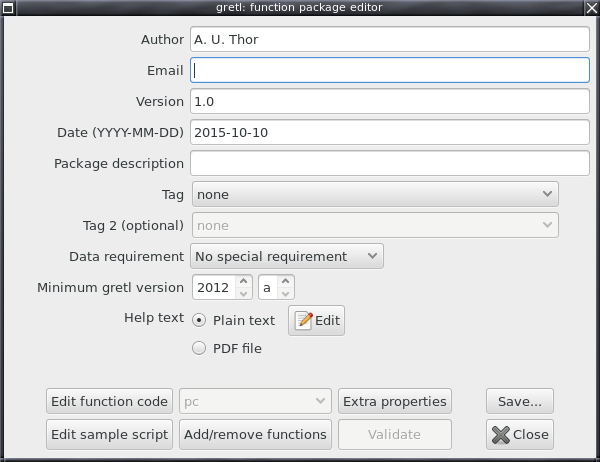
\includegraphics[scale=0.5]{figures/package_editor}
  \caption{The package editor window}
  \label{fig:package_editor}
\end{figure}

On clicking \textsf{OK} a second dialog should appear (see
Figure~\ref{fig:package_editor}), where you get to enter the package
information (author, version, date, etc.).  You should also enter help
text for the public interface.  You have a further chance to edit the
code of the function(s) to be packaged, by clicking on \textsf{Edit
  function code}.  (If the package contains more than one function, a
drop-down selector will be shown.)  

And you get to (in fact, you \textit{must}) add a sample script that
exercises your package.  This will be helpful for potential users, and
also for testing. For this package, a suitable sample script might
looks like this:
%
\begin{code}
include pcchange.gfn
open denmark.gdt
series pcLRM = pc(LRM)
print LRM pcLRM --byobs
\end{code}
%
where (a) we've decided that the package is to be called
\textsf{pcchange}, and (b) we're going to illustrate using S\o{}ren
Johansen's Danish macroeconomic data (included with the gretl
package). See section~\ref{sec:common-sample} for details on what's
required of a sample script.

At this point you should also consider the metadata items
\textsf{Minimum gretl version} and \textsf{Data requirement}.  You can
read all about these in section~\ref{sec:spec-basic}. For the moment,
suffice it to say that since the function code above doesn't do
anything exotic you may be OK leaving the minimum gretl version at its
default value, though if you want to check when some function or
command was introduced you can look at the gretl
ChangeLog.\footnote{See
  \url{http://gretl.sourceforge.net/ChangeLog.html}.} As for the data
requirement, well, percentage changes from observation to observation
probably don't make sense for cross-sectional data (which in most
cases can be ordered any old how, arbitrarily), so you might pull down
the list of options and select ``Time-series data.''

Clicking the \textsf{Save} button in the package editor window brings
up a little menu. For the present, it's just the first item,
\textsf{Save gfn}, that's relevant. If there's something missing from
your package specification at this point (e.g.\ no help text), you'll
get a nag box when you select this item. Otherwise you'll see a dialog
where you get to choose whether to save the \textsf{gfn} file to an
``installed'' location (see section~\ref{sec:installed}) or in some
other place; you are also prompted for a name for the package
(Figure~\ref{fig:gfnsave}). The package-name entry box will offer the
names of any suitable public functions as candidates (here \textsf{pc}
is the default). But you can type in some other name, and recall that
in our example the package should be called \textsf{pcchange} for
consistency with the sample script.

\begin{figure}[htbp]
  \centering
  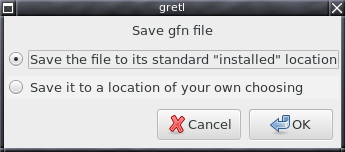
\includegraphics[scale=0.6]{figures/gfnsave}
  \caption{Where do you want your new package to go?}
  \label{fig:gfnsave}
\end{figure}

If you select the first option you will get feedback on where the gfn
file was actually written;\footnote{Technical note: this option will
  take care of saving the \textsf{gfn} to a named subdirectory of the
  relevant \texttt{functions} directory, if the specification includes
  PDF documentation or other additional files.} if you select the
second you'll get a regular File Save dialog box. The advantage of the
first choice is that the package will be found automatically by gretl.
However, if you're just experimenting and don't want to ``install''
the package yet, by all means choose a different location.

\subsection{Check your package!}

Before sharing your package with others, you must check that it
actually works, outside of the package-editing context. You need to
emulate the context of somebody who has installed your package from
scratch.

First off, that means that if you didn't choose to write your package
into a standard location at the step in section~\ref{sec:gui-create}
you should do so now. Use the ``Save...'' button in the GUI package
editor or see section~\ref{sec:cli-install} for other options.

Once your package is in the right place, close gretl then reopen it.
Now go to ``Tools, Function packages, On local machine''. If all has
gone OK so far, you should see the file you packaged and saved, with
its short description.  If you click on ``Info'' you get a window with
all the information gretl has gleaned from the package.  If you click
on the ``View code'' icon in the toolbar of this new window, you get a
script view window showing the actual function code. Fine.

Now, back to the ``Function packages'' window. Think for a moment: you
required time-series data (didn't you?) so you should know that a
double-click on your package will just offer the option of running
your sample script if time-series data are not loaded
(section~\ref{sec:gui-using}). And if you're following directions you
have no dataset open at present. OK, it's worth trying that; your
sample script really, really should work regardless
(section~\ref{sec:common-sample}), so go ahead and
double-click.\footnote{By the way, here's another thing: after loading
  the function(s) from the package, open the GUI console. Try typing
  \texttt{help pc}: the help text you entered should be presented.}

Now, if that went OK, let's next try a ``clean'' invocation of your
function. (Close and restart gretl if you've messed with your package
at all in the interim.)  First we'll load suitable data---preferably
something different from the sample script, for example the file
\texttt{np.gdt} (From Nelson and Plosser, also supplied with gretl
among the sample datasets, under the \textsf{Gretl} tab). We'll
compute the rate of change for the variable \texttt{iprod} via your
new function and store the result in a series named \texttt{foo}.

Return to ``Tools, Function packages, On local machine,'' find your
package, and double-click on it. A window similar to that shown in
Figure~\ref{fig:function_call} will appear.  Notice that the
description string ``Series to process,'' supplied with the function
definition, appears to the left of the top series chooser.

\begin{figure}[htbp]
  \centering
  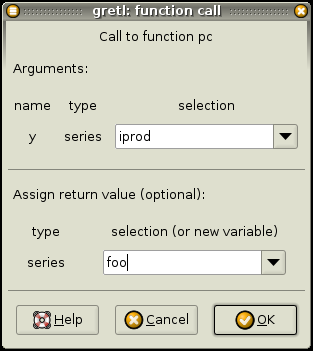
\includegraphics[scale=0.5]{figures/function_call}
  \caption{Using your package}
  \label{fig:function_call}
\end{figure}

Click \textsf{OK} and the series \texttt{foo} will be generated. Yay!
See Figure~\ref{fig:iprod_pc} (right-click on \texttt{foo} in the
gretl main window and choose \textsf{Time series plot}).

\begin{figure}[htbp]
  \centering
  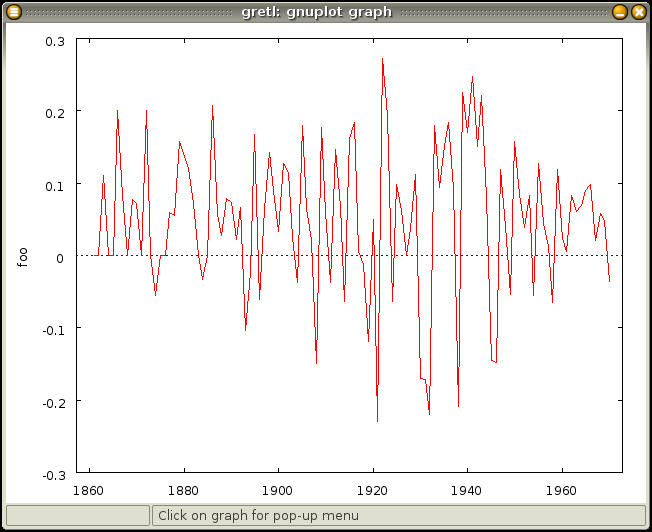
\includegraphics[scale=0.6]{figures/iprod_pc}
  \caption{Percent change in industrial production}
  \label{fig:iprod_pc}
\end{figure}

\section{Common requirements}
\label{sec:common-req}

Whether you're building a function package from the command line or
composing a package via the gretl GUI, certain requirements must be
met if your package is to be made available via the gretl server. Here
we spell out what's needed in regard to the help text and the sample
script.

\subsection{Help text}

This must give a clear (if brief) account, in English, of what the
package does, and also what each parameter does, for each public
function, insofar as explanation is reasonably required. (A boolean
\texttt{verbose} parameter probably doesn't need much if any comment,
but most parameters do need comment.)

If the help is not in PDF format (FIXME add cross-ref) it must be
encoded in UTF-8 (or plain ASCII, which is a proper subset of
UTF-8). We also recommend that lines of text are kept to close to 70
characters in width: some people may like to run gretl windows at
full-screen size, but many of us do not!

\subsection{Sample script}
\label{sec:common-sample}

This is crucial. The sample script \textit{must} work ``out of the
box'' on all platforms, and \textit{must not} take too long to
execute.

The sample script is what curious users are likely to run if they just
want to see what a package does and check that it's not broken. It's
what we gretl developers want to run for the same reasons, but also in
the process of regression-testing new gretl release candidates. It's
important that a gretl release doesn't break existing packages,
but we can't assess that if a package's sample script is broken in the
first place.

Here are the key things to watch out for in relation to sample
scripts:

\vspace{1ex}
\textbf{Include yourself}: Right at the top, the sample script
  must \texttt{include} the \texttt{gfn} file in question. This will
  never do any harm, and is needed when the script is run ``from
  scratch'', without the package being already loaded.  The name of
  the \texttt{gfn} file should be given without any added path, and
  without quotation marks, as in

  \texttt{include mypkg.gfn}

\vspace{1ex}
\textbf{Dataset}: If the package requires that a dataset be in
  place the sample script \textit{must} arrange for this in a portable
  manner. The options are as follows.
 \begin{enumerate}
 \item Open a data file that's supplied with the gretl distribution
   (that is, under the \textsf{Gretl}, \textsf{Greene} or
   \textsf{Ramanathan} tabs in the built-in datafile browser).
   But if none of the supplied data files are suitable, then
 \item construct an artificial dataset using the \texttt{nulldata}
   command and gretl's random-number generation facilities, or
 \item specify a downloaded data file using the \texttt{http} prefix
   with the \texttt{open} command, or
 \item include a suitable data file in your package---this requires
   that the package be in zip format.
 \end{enumerate}
 In the case of artificial data, the script should include a
 \texttt{set seed} command so that the results are reproducible. In
 the case of downloaded data the URL should be reasonably stable, not
 something that's likely to disappear or be moved before long.

 In \textit{no case} should a datafile be specified with a full path,
 as in
 \begin{code}
 open /usr/share/gretl/...
 open C:\Program Files\gretl\...
 \end{code}
  This is obviously not portable, and is never necessary when opening
  a supplied data file, given gretl's path-searching capability.

\vspace{1ex}  
\textbf{Execution time}: Some packages carry out Monte Carlo
  analyses and/or bootstrapping and we all know that such procedures
  are inherently time consuming. Nonetheless, a sample script should
  execute on current hardware in a reasonably short time---preferably
  less than 15 seconds and certainly less than a minute. Otherwise
  both casual users and testers will lose patience. If this means that
  only a ``toy'' example can be run, that's OK. The author can add
  comments to the script saying that this is just an illustration,
  serious use requires many more iterations. And/or one can add a more
  ``realistic'' invocation of the function(s), commented out, with a
  statement such as ``Uncomment this for a real test''.

\vspace{1ex}  
\textbf{Commenting out}: In some cases an author may wish to
  indicate alternative ways of calling his or her package. That's
  fine, but if an alternative call requires a dataset other than
  the one opened by the script it must be commented out; we don't
  want any lines in the sample script that will generate errors
  when the script is called ``as is''. 

\vspace{1ex}
The intent of the sample script in a gfn package is not just ``a rough
idea of how you might call this package'', or ``something that ran OK
for the author on some machine at some time'', but something that will
run for any user of gretl on any platform, without modification,
provided only that their gretl installation satisfies the stated
version requirement of the package.

\section{Gretl package idioms}
\label{sec:idioms}

The previous section set out certain basic requirements that must be
met if a package is to be published (on which see
section~\ref{sec:publish}). Nothing in the present section is a
requirement as such, but we urge you to take a look at our discussion
of the ``idioms'' that are found in many of the best packages. If your
package ``speaks gretl'' fluently that will give users a better
experience and make a more noteworthy contribution to the gretl
ecosystem.

Two main points are considered here (they often, but do not have to,
go together), namely offering a gretl bundle as the return value from
a packaged function, and offering placement of a function package on
one or other of the gretl menus. 

[FIXME: this section as a whole has a good deal of material that I
want to include, but it needs reworking -- at present it's 
mostly just ripped from my ``Addons and Bundles'' with minimal
changes. AC]

\subsection{Working with bundles}

The use of a bundle as the return type for a function allows it to
pass back a conveniently wrapped collection of information of various
kinds and dimensions. Furthermore, a package can contain functions
whose job is to access and process ``its own'' bundles, thereby
offering convenient GUI or scripting functionality for the user.

There's a close analogy between this facility and the built-in
handling of models in gretl. You specify a model via a dialog box, and
what happens? Execution burrows off into libgretl, where the
calculations are done and the results assembled into a data structure
called a \texttt{MODEL}, which is then returned to the GUI. The GUI
program then puts up a window displaying various aspects of the
model. In the background the full \texttt{MODEL} is ``attached'' to
the window, and the menu items in the window call functions that
access the underlying data structure to display things not shown by
default (e.g.\ the residuals), to make graphs (e.g.\ the residual
correlogram), to calculate diagnostic tests, and so on.

A function that returns a bundle can do just this sort of thing, and
wherever it's appropriate we recommend that this facility be
exploited.

Let's see how this works by reference to the \textsf{gig} package
(GARCH in gretl, written by Jack Lucchetti). The specification file
gig.spec contains three relevant entries:
%
\begin{code}
gui-main = GUI_gig
bundle-print = gig_bundle_print
bundle-plot = GUI_gig_plot
\end{code}
%
The first of these singles out \texttt{GUI\_gig} (among the many
public functions in the package) as the default interface for use
in the gretl GUI. [...]

% Commented extracts from gig.spec:

% \begin{itemize}
% \item \texttt{help = gig.pdf} : this line in the spec file tells gretl
%   that the help for \texttt{gig} is in PDF. Unlike plain-text help,
%   the specified file is not incorporated into the \texttt{gfn} file,
%   but is included in the package file \texttt{gig.zip}.
% \item \texttt{gui-main = GUI\_gig} : The \texttt{gui-main} key is
%   optional in a spec file, and is relevant only if the package
%   includes more than one public function. If a package has multiple
%   public functions and no \texttt{gui-main} is specified, then on
%   selecting the relevant GUI menu item the user will first be
%   presented with a drop-down list of functions. The effect of
%   \texttt{gui-main} is to single out a particular public function as
%   the entry point, hence by-passing the function listing and
%   streamlining the user experience.
% \item \texttt{bundle-print = gig\_bundle\_print} : The
%   \texttt{bundle-print} key is required for addons that return
%   bundles. It is used to specify a function that prints the contents
%   of bundles created by the package. The signature of the
%   function so designated must conform to a specific standard; see
%   below.
% \item \texttt{bundle-plot = GUI\_gig\_plot} : The \texttt{bundle-plot}
%   key is optional; it is used to specify a function that can produce
%   one or more types of plot based on the bundle returned by the
%   function. Again, this function (if given) must conform to a
%   standard.
% \end{itemize}

[XREF for details. Connecting text needed here.]

In \textsf{gig} we have:
%
\begin{verbatim}
  function void gig_bundle_print(bundle *model)
\end{verbatim}
%
and
%
\begin{verbatim}
  function void GUI_gig_plot(bundle *model, int ptype[0:1:0] \
                             "Plot type" {"Time series", "Density"})
\end{verbatim}

That is, \texttt{gig}'s basic \texttt{bundle-print} function has no
options, but its \texttt{bundle-plot} function has a control parameter
\texttt{ptype}. Note how the \texttt{ptype} parameter is set up: it
has a minimum value of 0 and a maximum of 1 (these options could be
extended), and 0 is the default. Further, the parameter is given a
name for display in the GUI, ``Plot type'', and it also has
strings---``Time series'' and ``Density''---associated with its two
possible numerical values. The latter strings will be used to populate
a menu on the window displaying a \texttt{gig} bundle.

Here's a sketch of how the whole apparatus works (i.e.\ a package
creates a bundle and the bundle is displayed in the GUI):

\begin{enumerate}
\item The user loads a time-series dataset, goes to the \textsf{/Model/Time
  series} menu, and selects \textsf{GARCH variants}.
\item Gretl loads the \texttt{gig} package (if it's not already loaded)
  and checks to see if it has a \texttt{gui-main} function
  specified. Yes, it does, so the argument-selection dialog for
  \texttt{GUI\_gig} is displayed directly.
\item The user makes appropriate selections in the dialog and clicks
  \textsf{OK}. (If she wants help she clicks \textsf{Help}, and is
  shown gig's PDF documentation.)
\item Gretl calls \texttt{GUI\_gig} and ``grabs'' the bundle that it
  returns.
\item Gretl looks up \texttt{gig}'s \texttt{bundle-print} function and
  invokes it on the bundle. The output from this function is then
  displayed in a GUI window.
\item When building this window, gretl reads the bundle's list of
  contents and creates a menu (UPDATE, toolbar) which enables the user
  to save specific items (matrices, series and so on) from the
  bundle. If the bundle is not already saved by name, this MENU also
  offers the option of saving the entire bundle ``as an icon''.
\item Also when building the bundle window, gretl checks if gig has a
  \texttt{bundle-plot} function. If so, a \textsf{Graph} menu
  (UPDATE!) is added; and if the \texttt{bundle-plot} function has
  options these are used to add items to the MENU. (If it has no
  options, there's just a single menu item.)
\end{enumerate}

SCREENSHOT

If the user closes the bundle window without saving the bundle itself,
the bundle is then destroyed. But if she saves it as an icon it
becomes accessible in the ``icon view'' window. Double-clicking on a
bundle icon again invokes its associated \texttt{bundle-print}
function, and the window described above is rebuilt. Bundles present
in the icon view are saved if the gretl session is saved to
file.\footnote{Once we've lost the immediate association between
  package and bundle, present when the bundle is first created via the
  GUI, how do we know which package to query when determining if (say)
  \texttt{bundle-plot} is applicable for a given bundle? The mechanism
  we use is that whenever a bundle is returned by a packaged function,
  we record the name of the package in a special member of the bundle
  structure.}

\subsection{Model-related packages}

The packages we've considered above share two characteristics: they
create and manipulate bundles, and they offer ``top-level''
functionality, in the sense that they naturally appear somewhere in
gretl's main menu tree.

It's also possible to write packages that do something interesting
based on data embedded in a gretl model---create a graph, run a test,
do a piece of analysis. Such functions (which may, but are not
required to, return bundles) have their proper place in menus on a
gretl model window, not the main menus.

Here's a brief overview of how such packages work.

\begin{enumerate}
\item The user estimates a model in the GUI and gretl constructs a
  window to show the output.
\item In the process of setting up the model-window menus, we check to
  see if any possibly relevant model-related addons are available.
\item If so, we run a ``pre-check'' (see below) to determine
  if the addon can handle the particular sort of model in
  question.
\item If yes, we add a menu item for the addon, and selecting
  this item pulls up a function call dialog for the addon.
\item The function is then executed in an environment in which gretl's
  model-related accessors, such as \verb|$uhat|, target the displayed
  model.
\end{enumerate}

Let's consider this in some more detail.  First, how do we tell if any
possibly relevant packages are available? UPDATED TEXT HERE.

Second, how do we tell, for each model-related addon, if it can
actually do something with the model we're displaying? 

REF MODEL-REQUIREMENT

For example, a given addon may offer an additional test that's
specific to models estimated via OLS, or to IV models.  Here we rely
on another ``special role'' function within the function
package. Parallel to the apparatus in a package spec file to identify
a function as (e.g.) a bundle-printer or bundle-plotter you can also
mark a function as a pre-checker, using the keyword
\texttt{gui-precheck}, as in

\begin{verbatim}
gui-precheck = foo_precheck
\end{verbatim}

XREF and reduce content here.

The \texttt{gui-precheck} function should \textit{not} be included in
the listing of public interfaces; it is intended only for internal use
by gretl. It must take no arguments and must return a scalar, which is
interpreted as an error code (0 for OK, non-zero for not OK). On
execution it has access to the \texttt{\$}-variables for the model in
question. Among these is the new accessor,
\verb|$command|, which gives the command-word for the estimator. So,
for example, the pre-check function for an addon which targets OLS
models might look like Code Example~\ref{code:precheck}.

\begin{script}[htbp]
\begin{scode}
function scalar ols_precheck (void)
  string cmd = $command
  if cmd != "ols"
    print "non-OLS model, can't handle"
    return 1
  else
    print "OLS model, OK"
    return 0
  endif
end function
\end{scode}
\caption{GUI pre-checking function}
\label{code:precheck}
\end{script}
%$

It's not necessary that such functions print anything. But anything
they do print goes to \texttt{stderr}. This can be useful for
debugging, but probably should not be retained in the ``production''
version of a package.

\subsection{Example: bandplot}
\label{sec:bandplot}

Model-related package example.

Creates a confidence band plot, that is, a plot displaying a
confidence band for the effect of a selected regressor in the context
of a multiple regression.  (Some more detail on what this means is
provided below.)  In GUI use, this package is intended to latch onto
windows displaying models estimated via OLS, attaching itself to the
\textsf{Graphs} menu.

Here's the relevant part of \texttt{bandplot.spec}: 

\begin{code}
description = Confidence band plot for regression effects
label = Confidence band plot
public = GUI_bandplot bandplot
gui-precheck = bandplot_precheck
gui-main = GUI_bandplot
help = bandplot.help
gui-help = bpgui.help
\end{code}

XREF!

The \texttt{label} and \texttt{gui-help} keywords in the spec file
merit discussion. First, the \texttt{label} entry gives a means of
controlling the label given to the package's menu item. Thus
\texttt{bandplot}'s menu item will read \textsf{Confidence band plot}.

The purpose of the optional \texttt{gui-help} keyword is to specify
help text to be presented in response to the \textsf{Help} button in a
dialog box. Note that in the online help for core gretl commands, a
distinction is made (maybe not quite as consistently as it should be)
between text to be shown for scripting use and text to be shown if the
user clicks on \textsf{Help}. The former may refer to option flags and
arguments, the latter to buttons and pull-down lists. The
\texttt{gui-help} spec file item extends this possibility to function
packages. The string to the right of the equals sign should give the
name of a plain text (UTF-8) file containing the GUI-specific help
text. 

Ref to bpgui.help.

Additional features helpful for this sort of thing.

First, besides the \texttt{[min:max:default]} fields for a function
parameter, you can add a fourth field to specify a ``step''. This
is used only for non-integer scalar parameters. To make the step value
active, the other three numerical fields must also be given. Example:

\begin{code}
function void foo (scalar clevel[0.5:0.99:0.95:0.01])
\end{code}

The effect of the above is that in the GUI the parameter
\texttt{clevel} will be represented by a ``spin-button'' with a
minimum of 0.5, a maximum of 0.99, an initial value of 0.95, and a
step or increment of 0.01 when the button is clicked. The step
specifier is ignored outside the context of a GUI function-call
dialog. Not specific to model-related packages.

Second, a facility specific to model-related packages, and in
particular to packages that target models carrying a list of
regressors. You can replace the \texttt{[min:max:default]} fields with
a single special symbol, \verb|[$xlist]|, as in

\begin{code}
function void foo (int xnum[$xlist])
\end{code}
%$

The effect is that in a GUI dialog the parameter \texttt{xnum} is
represented by a drop-down list showing the names of the regressors
(skipping the constant, if any).  Based on the user's selection from
the list, the argument is filled out with the 1-based index of the
position of the selected regressor in the array of coefficients. For
example, if the list of regressors is \texttt{const x1 x2 x3} then the
drop-down list will show \textsf{x1}, \textsf{x2} and \textsf{x3}, and
if the user selects \textsf{x2} the value 3 will be given to
\texttt{xnum}.

The idea is that if an addon wants to single out a regressor, much the
most user-friendly way of conveying this to the user is to show a list
of names. Yet there is no way that a package can arrange for this
directly; so we want a means of signalling to gretl that the list
should be constructed at runtime, based on the particular model.

Third, consider a package whose job is to produce a special graph
based on model data. By default, when a packaged function is invoked
via the GUI a window is opened showing the command along with any
printed output, but for graph-only output such a window is superfluous
and potentially confusing.  You can now suppress the text window by
inserting a special comment into the code of the function in question,
namely

\begin{code}
## no-print ##
\end{code}

UPDATE: ref no-print list in spec file or GUI Extra props.


\section{Publishing a package}
\label{sec:publish}

If you decide that you'd like to publish a package---that is, make it
available via the channels described in
section~\ref{sec:acquire}---here's the procedure.

Preliminary: please double-check your package to ensure you have met
the requirements in section~\ref{sec:common-req}. This will save
everyone's time.

\subsection{Uploading to the gretl server}

If you don't already have a login to the gretl package server, you
need to begin by creating one (please note, this is not the same thing
as a sourceforge login). The URL will be given to you by gretl if you
go to upload a package via the GUI, but for reference it's
\url{http://gretl.ecn.wfu.edu/cgi-bin/apply/}.

With a login in hand, you can upload a package via the GUI package
editor: under the \textsf{Save...} menu you'll find an \textsf{Upload
  to server} option. Alternatively you can use the \app{curl} program:
this is standard kit on platforms other than MS Windows, but also
available for Windows via
\url{http://curl.haxx.se/download.html}. Below is an example shell
script for uploading a plain \textsf{gfn} file. Of course you'd have
to fill out the first three lines appropriately.

\begin{code}
user=your_gretl_login
password=your_gretl_password
pkg=/path/to/your_package.gfn

savename=`basename $pkg`
curl -F login="${user}" -F pass="${password}" \
-F "pkg=@${pkg};filename=${savename};type=text/plain;charset=utf-8" \
http://ricardo.ecn.wfu.edu/gretl/cgi-bin/gretldata.cgi
\end{code}
%$

Uploading a zip package via the GUI is no different from uploading a
plain \textsf{gfn}: gretl handles the details, producing a zipfile in
the background. But if you're using the command line the process is a
bit different. You need to create the zipfile first, then use a
modified version of the \textsf{curl} upload script shown above.

One way of building the zipfile is to use the \cmd{makepkg}
command in the gretl console or in \app{gretlcli}, as in
%
\begin{code}
makepkg mypkg.zip
\end{code}
%
When the argument to \cmd{makepkg} is a filename with the \textsf{zip}
extension, gretl will do one of two things:
\begin{itemize}
\item If a matching \textsf{gfn} file is found, this will be used the
  as the basis for the zipfile, with other components pulled in as
  needed.
\item Failing that, if a matching \textsf{spec} file is found (plus
  the other files that it references), gretl will first build the
  \textsf{gfn}, then build the zipfile wrapper.
\end{itemize}

Alternatively you can use the command-line \app{zip} program to do the
job by hand, as in
%
\begin{code}
zip -r mypkg.zip mypkg
\end{code}
%
where we assume that \texttt{mypkg} is a subdirectory of the current
working directory containing everything that's needed for the package,
laid out as described in chapter~\ref{chap:zipfile}. 

For the modified \app{curl} invocation that is needed to upload a
zipfile, see Example~\ref{ex:curl-zip}.

\begin{script}[htbp]
  \centering
  \caption{Shell script for uploading zipfile}
  \label{ex:curl-zip}
\begin{scode}
user=your_gretl_login
password=your_gretl_password
pkg=/path/to/your_package.zip

bytes=`stat $pkg --printf="%s"`
savename=`basename $pkg`
echo "Uploading $pkg ($bytes bytes) as $savename ..."

curl -F login="${user}" -F pass="${password}" -F datasize="${bytes}" \
-F "pkg=@${pkg};filename=${savename};type=application/x-zip-compressed" \
http://ricardo.ecn.wfu.edu/gretl/cgi-bin/gretldata.cgi
\end{scode}
\end{script}
%$

Even if you build your package via the command line, gretl can help
with the uploading, if you prefer: in the main window, go to ``Tools,
Function packages, Upload package'' and choose the package to
upload. The file selection dialog will offer a choice of looking for
\textsf{gfn} or \textsf{zip} files. Please note: if your package is
supposed to contain PDF documentation or additional files, you must
build the zip file and upload that, not the plain \textsf{gfn}.

\subsection{Staging}

When your package is successfully uploaded, it first goes into a
``staging'' area on the server, and the gretl developers who are
responsible for package-checking are notified by email. Before too
long, hopefully, you should hear from one of the developers, with a
response of Accept, Reject, or Revise and Resubmit.

Typically, packages will be rejected only if they are considered too
trivial, if it turns out that they're really just duplicating
functionality that's already available in gretl, or if they clearly
make no attempt to comply with the stated requirements (section
\ref{sec:common-req} again). Revise and Resubmit is a likely response
if your package seems basically sound but some improvements are
warranted.

Once your package is accepted it is moved out of staging and will
appear in the public package listing, both within gretl (``On
server'') and via the web interface.


\section{Maintaining a package}
\label{sec:maint}

FIXME: This section should talk about issues arising in relation to
the maintenance of an existing package. Use of CLI and GUI and
cross-over between the two. Avoid reverting any changes made by
package admins to fix breakage in prior versions (tho' maybe that
should never happen?).


\chapter{Package specification details}
\label{chap:specfile}

Here we list and explain the usage of all the currently allowed
elements in the specification of a function package. We focus on the
\textsf{spec} file (from which a gretl function package may be
constructed by command-line means) but we also indicate the
representation of each specification element in the GUI package
editor.

We begin with a few general points on the \textsf{spec} file. Each
entry in this file takes the form

\texttt{keyword =} \textsl{value(s)}

Where multiple values are allowed, they should be separated by
spaces. An entry can be continued over more than one line if required,
using a trailing backslash (\verb+\+) as the continuation
character. Blank lines are ignored, as are lines beginning with the
hash mark (\texttt{\#}), which can be used to insert comments.  As
usual with gretl files, any non-ASCII characters should be UTF-8
encoded.

\section{Basic elements}
\label{sec:spec-basic}

The elements described in the section apply to all function packages,
whether or not they offer an interface specifically designed for
use via the gretl GUI and whether or not the main public function(s)
return a gretl bundle.

Elements in the first block below are all represented in the upper
panel of the GUI package editor window (see
Figure~\ref{fig:package_editor}).

\begin{description}

\item \texttt{author} (required): The name of the author of the
  package. Multiple names may be given, separated by ``and'', although
  note that this string may be truncated for presentation purposes in
  some contexts.

  \vbusage{} \verb|author = Riccardo "Jack" Lucchetti and Allin Cottrell|

\item \texttt{email} (required): The email address to which
  correspondence should be directed. Only one address should be given.

  \vbusage{} \verb|email = cottrell@wfu.edu|

\item \texttt{version} (required): The version number for the package
  release. This should be parseable as an integer or floating-point
  number (in the \textsf{C} locale). That is, it should contain only
  digits and at most one dot (\texttt{.}).

  \ttusage{version = 1.2}

\item \texttt{date} (required): The date on which the release was
  prepared, in ISO 8601 format, \textsf{YYYY-MM-DD}.

  \ttusage{date = 2015-03-28}

\item \texttt{description} (required): A short plain-text (UTF-8)
  string describing what the package does.

  \ttusage{description = logit/probit marginal effects}

 \item \texttt{min-version} (required): The minimum gretl version on
   which the package is supported, format \textsf{M.N.P} (three
   numbers separated by two dots). Ideally, this should truly be the
   first gretl version on which the package will run OK, but if in
   doubt it is preferable to specify a later version (users can
   always update) rather than an earlier one (on which the package
   might fail and give the user a bad impression).

   \ttusage{min-version = 1.9.12}

\item \texttt{data-requirement} (optional): If this element is
  supplied, it must be one of the following strings:
  \texttt{no-data-ok}, \texttt{needs-time-series-data},
  \texttt{needs-qm-data} (meaning, quarterly or monthly time-series
  data), or \texttt{needs-panel-data}. Note that the \textit{default}
  requirement is that a dataset of some sort is in place (cross
  sectional, time series or panel). If your function does not take any
  series or list arguments (for example, it does something with
  matrices), you should use \texttt{no-data-ok} to indicate that a
  dataset is not required.

  \ttusage{data-requirement = needs-panel-data}

\end{description}

The remaining ``basic'' elements are represented in the GUI
in various ways, as described below.

\begin{description}

\item \texttt{public} (required): A list of names of the public
  interfaces offered by the package.

  \vbusage{} \verb|public = GUI_lp_mfx lp_mfx_print mlogit_mfx \| \\
           \verb|                   mlogit_dpj_dx ordered_mfx |

  In the GUI this list can be accessed and modified via the
  \textsf{Add/Remove functions} button.

\item \texttt{sample-script} (required): the name of a hansl
   script (\texttt{.inp}) file that serves as examplar for use
   of the package.

   \ttusage{sample-script = keane-mfx.inp}

   GUI: access and edit via the \textsf{Edit sample script} button.

 \item \texttt{help} (required): The name of the file in which
  Help for this package can be found. This should either be a 
  plain text (UTF-8) file, in which case the filename suffix
  doesn't really matter---although we suggest \texttt{.txt}---or a
  PDF file, in which case the suffix must be \texttt{.pdf}. 

  \vbusage{} \verb|help = lp-mfx_help.txt|

  GUI: The help text is found in the lower panel of the main package
  editor window. To specify PDF documentation you put a special entry
  into this panel, on the pattern

  \texttt{pdfdoc:mypkg.pdf}

  where \texttt{mypkg} should be replaced by the actual package name.

\end{description}

\section{GUI-related elements}
\label{sec:spec-gui}

The elements described in this section are applicable only if at least
one function in the package is designed to be called via gretl's
graphical interface. In the GUI package editor these elements are
shown in one or other tab of the the window that appears on clicking
the \textsf{Extra properties} button.

\begin{description}

\item \texttt{menu-attachment} (optional): Specifies a place within
  the gretl menu system under which the package should be made
  available. At present packages can attach to menus (a) in the main
  gretl window and (b) in windows displaying model estimates
  (only). In specifying a \texttt{menu-attachment} these are
  represented by the strings \texttt{MAINWIN} and \texttt{MODELWIN}
  respectively. The ``path'' to the entry for your package should
  start with one of these identifiers; this should be followed by one
  or more slash-separated elements, using the internal representation
  of the menu tree in \texttt{gretlmain.xml} or
  \texttt{gretlmodel.xml}---these XML UI files can be found in the
  gretl source package or in CVS.\footnote{See
    \url{http://gretl.cvs.sourceforge.net/viewvc/gretl/gretl/gui2/}}

  \ttusage{menu-attachment = MODELWIN/Analysis}

\item \texttt{label} (conditionally required): A very short string
  that can be displayed in a GUI menu. This is relevant only if the
  package specifies a \texttt{menu-attachment}, in which case it is
  required.

  \ttusage{label = Marginal effects}

\item \texttt{gui-main} (optional): This entry is relevant only if a
  package offers more than one public interface. Its effect is to
  select one particular interface when a user accesses the function
  package via the gretl GUI (other public interfaces can be selected
  via the command line if the user so chooses). If a package offers
  multiple public interfaces and \texttt{gui-main} is \textit{not}
  specified, the user will be given a choice of interfaces whenever he
  or she calls the package. (If a package offers only one public
  interface, we can think of this as implicitly its ``gui-main''.)

  \vbusage{} \verb|gui-main = GUI_lp_mfx|

\item \texttt{gui-help} (optional): The name of a UTF-8 file
  containing GUI-specific help text, to be shown when the user
  clicks on \textsf{Help} in a dialog box representing the
  package. Such text may make reference to buttons, pull-down lists
  and the like rather than using language appropriate to command-line
  usage.

  \ttusage{gui-help = bpgui.help}

\item \texttt{menu-only} (optional): A list of public interfaces (in
  practice, probably only one) that are specifically designed to be
  called from a suitable GUI menu and that should \textit{not} be
  offered via the browser for installed packages. If any function
  falls in this category it's likely to be the one designated as
  \texttt{gui-main}.

  \vbusage{} \verb|menu-only = GUI_lp_mfx|

\item \texttt{model-requirement} (optional): When the ``gui-main''
  function of a package is designed to be called from a menu in a
  gretl model-output window, this element can be used to indicate that
  only models of a certain type are supported (and therefore the
  package will shown only for such models).  The right-hand value
  should be the gretl command-word corresponding to the supported
  estimator. See also \texttt{gui-precheck}.

  \ttusage{model-requirement = tobit}

\item \texttt{gui-precheck} (optional): Applies only when a
  \texttt{menu-attachment} is specified. This element identifies a
  function to be called to check whether the package is supported in
  context.  It offers a more flexible testing mechanism than
  \texttt{model-requirement}.

  The \texttt{gui-precheck} function should not be included in the
  listing of public interfaces; it is intended only for internal use
  by gretl. It must take no arguments and must return a scalar. On
  execution it has access to all the \texttt{\$}-accessors for the
  model in question. On this basis the function should return 0 if the
  model is supported, non-zero otherwise.

  \vbusage{} \verb|gui-precheck = lp_mfx_precheck|

\item \texttt{no-print} (optional): A list of public interfaces that
  are not designed to print anything.  Consider, for example, a
  package whose job is to produce a special graph based on model data.
  By default, when a packaged function is invoked via the GUI a window
  is opened showing the command along with any printed output, but for
  graph-only output such a window is superfluous and potentially
  confusing. You can suppress the text output window by adding such a
  function to the \texttt{no-print} list.

\end{description}

\section{Bundle-related elements}
\label{sec:spec-bundle}

The elements described below are applicable only if at least one
public function in the package returns a bundle. In the GUI package
editor these appear under the \textsf{Special functions} tab in the
\textsf{Extra properties} window.

\begin{description}

\item \texttt{bundle-print} (optional): Identifies a given function
  (which must be a public interface) that can be used to print the
  content of a bundle produced by the package.

  \vbusage{} \verb|bundle-print = oddsratios_print|

\item \texttt{bundle-plot} (optional): Identifies a given function
  (which must be a public interface) that can be used to produce some
  sort of plot or graph using the content of a bundle produced by the
  package.

  \vbusage{} \verb|bundle-plot = Brown_print|

\item \texttt{bundle-test} (optional): Intended for identifying a
  function that performs some sort of statistical test based on
  a bundle's content. Unused at present.

\item \texttt{bundle-fcast} (optional): Intended for identifying a
  function that generates a forecast based on a bundle's
  content. Unused at present.

\item \texttt{bundle-extra} (optional): Unused at present.

\end{description}

Functions selected for the special bundle-related roles must conform
to a definite standard, as follows:
\begin{itemize}
\item The first argument must be a bundle-pointer.
\item The second argument, if present, must be an \texttt{int} that
  controls the function's behavior in some way, and it must have a
  specified default value.
\item Any further arguments should also have default values (meaning
  that they can be omitted).
\end{itemize}

Taking the \textsf{gig} package as an example, we have:
%
\begin{verbatim}
  function void gig_bundle_print(bundle *model)
\end{verbatim}
%
and
%
\begin{verbatim}
  function void GUI_gig_plot(bundle *model, int ptype[0:1:0] \
                             "Plot type" {"Time series", "Density"})
\end{verbatim}

That is, \textsf{gig}'s \texttt{bundle-print} function has no options,
but its \texttt{bundle-plot} function has a control parameter
\texttt{ptype}. Note how this parameter is set up: it has a minimum
value of 0 and a maximum of 1 (these options could be extended), and 0
is the default. Further, the parameter is given a name for display in
the GUI, ``Plot type'', and it also has strings---``Time series'' and
``Density''---associated with its two possible numerical values. The
latter strings will be used to populate a menu on the window
displaying a \textsf{gig} bundle.

\section{Extra elements}
\label{sec:spec-extra}

At present there is only one spec file entry in this category; in the
GUI package editor it appears under the \textsf{Data files} tab in the
\textsf{Extra properties} window.

\begin{description}

\item \texttt{data-files} (optional): Specifies extra files that
  should be included in the package. Use of this option implies that
  the package should take the form of a zipfile. See
  chapter~\ref{chap:zipfile} for details.

  \ttusage{data-files = special.gdt extradir}

\end{description}

\chapter{Zip package details}
\label{chap:zipfile}

The zip format was originally supported only for officially recognized
``addons'' such as \textsf{gig} and \textsf{SVAR}, but since gretl
1.10.1 it is also supported for contributed function packages.

\section{Basic specification}

At minimum, a zip package must contain a top-level directory with the
same name as the package itself, and this directory must contain the
\texttt{gfn} file. Suppose the name of the package is \textsf{mypkg};
in that case the minimal zipfile looks like this (as shown by the
\textsf{unzip} program with its \texttt{-l} option to list the
contents of an archive):
%
\begin{code}
Archive:  mypkg.zip
  Length      Date    Time    Name
---------  ---------- -----   ----
        0  2015-06-07 10:54   mypkg/
    10708  2015-06-07 10:54   mypkg/mypkg.gfn
---------                     -------
    10708                     2 files
\end{code}

There would be little point in creating a package with just the
content shown above; the advantage of the zipfile format lies in the
possibility of including extra materials that cannot be stuffed into
a \texttt{gfn} file. Such materials fall into four main categories:

\begin{itemize}
\item PDF documentation. This should take the form of a pdf file with
  the same basename as the package, included in the top-level package
  directory. Thus, to continue the example above, the directory
  \texttt{mypkg} might contain \texttt{mypkg.pdf} as well as
  \texttt{mypkg.gfn}.
\item Data to support a sample script. This answers the case where a
  package author wishes to use specific data, not present in the gretl
  distribution, with his or her sample script. For example, the
  \textsf{almonreg} package contains the datafile \texttt{almon.gdt}
  to permit replication of Shirley Almon's original modeling.
\item Data for internal use. For example, gretl matrix files
  containing tables of critical value for some hypothesis test
  implemented by the package.
\item Extra examples: scripts and/or data files that go beyond the
  required sample script to give users a full sense of the scope and
  usage of a complex package.
\end{itemize}

\section{Example: \textsf{almonreg}}

Here's a fairly simple real case, the \textsf{almonreg} package:
%
\begin{code}
Archive:  almonreg.zip
  Length      Date    Time    Name
---------  ---------- -----   ----
        0  02-12-2015 13:27   almonreg/
    55861  02-12-2015 13:27   almonreg/almonreg.pdf
     4409  02-12-2015 13:27   almonreg/almonreg.gfn
     1969  02-12-2015 13:27   almonreg/almon.gdt
---------                     -------
    62239                     4 files
\end{code}

The relevant portion of the \textsf{almonreg} spec file, calling for
inclusion of the PDF and gdt files, reads thus:
%
\begin{code}
help = almonreg.pdf
data-files = almon.gdt
\end{code}

Note that when the \textsf{almonreg} sample script opens the data file
\texttt{almon.gdt} it must employ the \option{frompkg} option to tell
gretl where to find the file:
%
\begin{code}
open almon.gdt --frompkg=almonreg
\end{code}

\section{Example: \textsf{GHegy}}

Another illustration: Ignacio D\'iaz-Emparanza's \textsf{GHegy}
package (abbreviated):
%
\begin{code}
Archive:  GHegy.zip
  Length      Date    Time    Name
---------  ---------- -----   ----
        0  2015-03-12 13:51   GHegy/
    18610  2015-03-12 13:51   GHegy/GHegy.gfn
        0  2015-03-12 13:51   GHegy/coeffs/
    52960  2015-03-12 13:51   GHegy/coeffs/CFt_c_fijo.mat.gz
    53276  2015-03-12 13:51   GHegy/coeffs/CFt_cD_fijo.mat.gz
    42990  2015-03-12 13:51   GHegy/coeffs/Ct2_c_BIC.mat.gz
    ...    ...                ...
---------                     -------
  3798063                     83 files
\end{code}

In this instance we don't have PDF documentation, but we do have a
large number of gzipped gretl matrix files, holding response-surface
coefficients by means of which the package is able to compute
$P$-values for the HEGY seasonal unit-root test. The relevant
spec file clause is
%
\begin{code}
data-files = coeffs
\end{code}
%
Note that putting \texttt{coeffs} (the name of a directory) into the
data-files list ensures that all the contents of this directory will
be included in the zip package. At run time \textsf{GHegy} can access
its matrix files using the accessor variable
\verb|$pkgdir|, which will expand to the appropriate
platform-dependent path, as in
%
\begin{code}
string matname = sprintf("%s/coeffs/CFt_c_fijo.mat.gz", $pkgdir)
matrix C = mread(matname)
\end{code}

\section{Example: \textsf{HIP}}

Our final illustration is the \textsf{HIP} package (which now has
official ``addon'' status), written by Jack Lucchetti and Claudia
Pigini. Looking in the zipfile we see:
%
\begin{code}
Archive:  HIP.zip
  Length      Date    Time    Name
---------  ---------- -----   ----
        0  03-19-2015 19:58   HIP/
        0  03-19-2015 19:58   HIP/examples/
    75210  03-19-2015 19:58   HIP/examples/camtriv_chap14.gdtb
      657  03-19-2015 19:58   HIP/examples/camtriv_chap14.inp
     1941  03-19-2015 19:58   HIP/examples/MonteCarlo.inp
   383278  03-19-2015 19:58   HIP/HIP.pdf
    27691  03-19-2015 19:58   HIP/HIP.gfn
---------                     -------
   488777                     7 files
\end{code}

We have PDF documentation plus an \texttt{examples} directory. The
latter is special: if a zip package contains a directory named
\texttt{examples} (\textit{exactly} that, in English and all lower
case), then in the GUI function package browser the ``Resources...''
button (open folder icon) and menu item become active. Selecting this
item opens a file dialog pointing at the examples directory, from
which you can open any scripts or datafiles that are provided. These
are intended to supplement the required sample script.


\bibliography{gretl}

\end{document}


